\documentclass[conference]{IEEEtran}

\usepackage{cite}
\usepackage{amsmath,amssymb,amsfonts}
\usepackage{algorithmic}
\usepackage{graphicx}
\usepackage{textcomp}
\usepackage{xcolor}
\def\BibTeX{{\rm B\kern-.05em{\sc i\kern-.025em b}\kern-.08em
    T\kern-.1667em\lower.7ex\hbox{E}\kern-.125emX}}
\begin{document}

\title{Progetto B2: Algoritmi di Mutua Esclusione Distribuita in Go\\}

\author{\IEEEauthorblockN{Sara Da Canal\\
\textit{matricola 0316044}}
\IEEEauthorblockA{\textit{Corso di Sistemi Distribuiti e Cloud Computing} \\
\textit{Laurea Magistrale in Ingegneria Informatica,
Università di Roma Tor Vergata} \\
s.saradacanal@gmail.com}
}

\maketitle

\begin{abstract}
Questo documento ha l'obiettivo di descrivere la realizzazione di un sistema di mutua esclusione distribuita e le scelte progettuali effettuate durante la realizzazione.
Verranno presentati l'architettura del sistema e gli algoritmi selezionati per l'implementazione, evidenziando i motivi di queste scelte e le sfide incontrate durante la realizzazione del progetto. 
\end{abstract}


\section{Introduzione}
Lo scopo di questo progetto è creare un sistema di mutua esclusione distribuita, che offre l'implementazione di diversi algoritmi:
\begin{itemize}
\item Ricart-Agrawala, algoritmo totalmente distribuito e basato su autorizzazione
\item Maekawa, algoritmo totalmente distribuito e basato su quorum
\item Un algoritmo basato su un token centralizzato, per cui è necessaria la presenza di un coordinatore
\end{itemize}
Il progetto prevede un sistema di registrazione, responsabile di mettere in contatto i diversi peer tra di loro e di avviare il coordinatore per l'algoritmo centralizzato.
\`E possibile impostare il numero di peer con cui avviare il sistema e quale algoritmo usare, e anche simulare diverse condizioni di ritardo della rete tramite un parametro \textit{delay}, che genera del ritardo per l'invio dei messaggi.
Il progetto prevede un parametro \textit{verbose} per consentire il debugging e dei test, che controllano che gli algoritmi implementati garantiscano mutua esclusione, fairness e liveness. Il sistema utilizza Docker, ognuno dei peer è incapsulato in un diverso container, la cui orchestrazione viene gestita tramite docker-compose. Il sistema è poi stato deployato su un'istanza EC2

\section{Tecnologie adottate}
I seguenti linguaggi e framework sono stati usati per lo sviluppo del progetto:
\begin{itemize}
\item \textbf{Go}: linguaggio usato per l'implementazione del sistema, come richiesto dalle specifiche
\item \textbf{Docker}: è usato come supporto alla virtualizzazione.
\item \textbf{Docker-compose}: è usato per creare una rete tra i singoli container.
\item \textbf{go-RPC}: per la comunicazione tra diversi container è stato usato il supporto nativo di go alle RPC tramite il package "net/rpc".
\item \textbf{EC2}: è stato effettuato il deploy dell'applicazione su una macchina virtuale creata usando questo servizio.
\end{itemize}

\subsection*{Utilizzo di go-RPC}

Scegliere quale metodo utilizzare per la comunicazione tra diversi processi è stato uno dei punti focali del progetto. Infatti, go offre un supporto nativo alle RPC, che però presenta delle limitazioni. L'alternativa sarebbe usare le GRPC, che permettono di comunicare anche tra client scritti in linguaggi diversi. Nonostante le GRPC sono sicuramente molto più versatili, soprattutto nella creazione di applicazioni a microservizi, il supporto nativo che go offre ha il vantaggio di essere molto semplice da usare e offrire un mezzo di comunicazione affidabile tra diversi programmi scritti in golang, quindi anche se non completo per tutte le situazioni il package "net/rpc" è più che adatto agli scopi di questo progetto.

\section{Implementazione degli algoritmi}

Nella scelta degli algoritmi la prima cosa che ho preso in considerazione è stato di scegliere tre algoritmi appartenenti a categorie differenti, uno di autorizzazione, uno basato su token e uno su quorum, in modo tale da non implementare algoritmi troppo simili tra di loro. Algoritmi basati su token distribuito, per quanto esistenti, non sono efficienti, mentre l'algoritmo basato su token centralizzato è uno dei più semplici e funzionali tra gli algoritmi centralizzati, motivo per cui è stato scelto. Dovendo poi scegliere un algoritmo distribuito per ognuna delle altre categorie, sono stati scelti Ricart-Agrawala e Maekawa perché rispettivamente i più popolari per ogni categoria
 
\subsection{Ricart-Agrawala}

Questo algoritmo sfrutta un clock logico scalare per l'ordinamento delle richieste. Un peer che utilizza questo algoritmo può trovarsi in tre stati differenti: 
\verb|HELD| (il peer si trova in sezione critica), \verb|WANTED| (Il peer ha fatto richiesta per la sezione critica) e \verb|RELEASED| (Il peer non si trova in sezione critica ne desidera entrarvi).
Tra di loro i peer si mandano solo due tipi di messaggi, \verb|request| e \verb|reply|: ogni volta che un peer vuole entrare in sezione critica invia un messaggio di \verb|request| a tutti gli altri partecipanti al gruppo di mutua esclusione, specificando il proprio id e il proprio clock. Ogni volta che un peer esce dalla sezione critica, invia un messaggio di \verb|reply| per tutte le richieste che ha messo in coda. Quando invece arriva un messaggio di \verb|request| a cui va data risposta immediatamente (questo avviene quando il peer si trova in stato \verb|RELEASED|, oppure in stato \verb|WANTED| ma la sua richiesta è successiva a quella ricevuta), non viene inviato un messaggio di risposta separato ma viene sfruttato il fatto che le go-RPC prevedono una risposta immediata sullo stesso canale di comunicazione. Per poter entrare in sezione critica, ogni peer deve avere l'autorizzazione di ogni altro. Un peer concede l'autorizzazione se si trova in stato \verb|RELEASED| o se si trova in stato \verb|WANTED| e il clock della sua richiesta è maggiore rispetto alla richiesta arrivata. I clock vengono confrontati secondo una relazione di ordine totale,  che per clock logici scalari significa ordinamento secondo il clock e nel caso di parità si considera minore la richiesta provenente dal peer con id minore.

\subsection{Token centralizzato}

Questo algoritmo richiede la presenza di un coordinatore che si occupa di gestire il token e inviarlo ai peer. Il token deve essere unico, chi possiede il token infatti può entrare in sezione critica. Il coordinatore non deve essere uno dei peer, perché non invia richieste per entrare in sezione critica. L'algoritmo si basa su un clock logico vettoriale, che ogni peer aggiorna usando i messaggi di programma. Il coordinatore si basa su questo clock per decidere a chi inviare il token. I peer inviano due tipi di messaggi verso il coordinatore: \verb|request| per entrare in sezione critica, a cui il coordinatore risponde immediatamente se ha il token, e messaggi di \verb|release| del token una volta completata la sezione critica. Quando il coordinatore riceve di nuovo il token, seleziona la prima richiesta eleggibile tra quelle in coda e invia un messaggio di \verb|reply| con il token al peer corrispondente. I peer inviano anche i messaggi di programma agli altri partecipanti al gruppo di mutua esclusione: ogni volta che inviano una richiesta, mandano il proprio clock. Quando un peer riceve un messaggio di programma aggiorna il proprio clock. Grazie ai messaggi di programma, un peer può informare il coordinatore di quante e quali richieste ha visto nel momento in cui invia la propria. Il coordinatore non considera una richiesta eleggibile finché non ha servito tutte quelle viste in precedenza. Questo significa che il clock vettoriale ha lunghezza uguale al numero dei peer, e una richiesta è eleggibile se tutte le componenti del suo clock esclusa quella riferita al peer che l'ha inviata sono minori o uguali rispetto alle componenti del clock del coordinatore. Il coordinatore aggiorna il proprio clock quando invia il token a un peer, aggiornando solo la componente che corrisponde al peer a cui ha risposto con il valore della richiesta a cui ha risposto.

\subsection{Maekawa}

Questo algoritmo basato su quorum è senza dubbio quello che presenta più sfide implementative tra i tre selezionati. Come Ricart-Agrawala, anche qui un peer può essere in stato \verb|HELD|, \verb|WANTED| o \verb|RELEASED|, ma essendo basato su quorum non richiede l'autorizzazione di tutti i membri del gruppo di mutua esclusione per entrare in sezione critica ma solo di una parte, il suo quorum appunto. Una delle difficoltà presentate da questo algoritmo è il fatto che presenta molti tipi di messaggi diversi, soprattutto se andiamo a considerare i messaggi relativi all'evitare i dead-lock, che nella versione base dell'algoritmo possono verificarsi. Ogni peer ha un solo voto: se gli arriva un messaggio di \verb|request|, da risposta affermativa se il suo voto è disponibile, mette in coda altrimenti. Quando gli arriva un messaggio di \verb|release|, il suo voto torna disponibile, a questo punto può andare a prendere il primo messaggio nella coda e inviare il voto con un messaggio di \verb|reply|. Per evitare i dead-lock è necessario aggiungere un quarto messaggio non presente negli altri algoritmi, il messaggio di \verb|inquire|: se un peer che ha già votato riceve una richiesta con numero di sequenza minore di tutte quelle in coda e della richiesta votata, manda al peer per cui ha votato un messaggio di \verb|inquire|. Un peer che riceve un messaggio di \verb|inquire| lo ignora se ha ricevuto tutti i voti per entrare in sezione critica, se invece ha avuto risposte negative rinuncia al suo voto, dando precedenza alla nuova richiesta. La seconda grande difficoltà di questo algoritmo è quella di calcolare il quorum, che è stata risolta usando un algoritmo per il calcolo del quorum in un grafo completo e indiretto descritto nel paper \cite{b1}. Questo algoritmo fornisce una maschera di bit, che, shiftata, può essere usata per ottenere n quorum diversi per n peer. La maschera viene calcolata in base al numero di peer dal sistema di registrazione e inviata ai peer, poi ogni peer usa la maschera ricevuta per calcolare il proprio quorum, shiftandola in base che il primo elemento del quorum sia sempre il peer che effettua il calcolo. In questo modo ogni peer ha un quorum diverso e che comprende anche il peer stesso, condizione utile per minimizzare il numero di messaggi inviati. L'algoritmo assicura che l'intersezione tra i quorum non sia mai nulla, ma non sempre riesce a raggiungere la soluzione ottima, quindi il minimo numero di peer per ogni quorum. Per stabilire la precedenza tra richieste anche questo algoritmo, come Ricart-Agrawala, si basa su un clock logico scalare.

\subsection*{Gestione della sezione critica}

Dato che è d'interesse per il progetto l'implementazione degli algoritmi per entrare in sezione critica, mentre concretamente una vera e propria sezione critica non esiste, è stata semplicemente implementata facendo si che il peer in sezione critica sia in fase di sleep per un certo tempo prima di rilasciarla. In particolare, la sleep viene effettuata per un massimo di 10 secondi.

\section{Sistema di registrazione}

Il sistema di registrazione all'avvio prende in input quale algoritmo usare e quanti peer parteciperanno all'esecuzione dell'algoritmo. Il numero di peer è necessario perché il registratore aspetta di aver raggiunto il numero di peer specificato, salva in una lista gli indirizzi a cui è possibile raggiungere questi peer e quando la lista è completa la invia ai peer. Inoltre assegna ad ogni peer un id, corrispondente alla sua posizione nella lista. Nel caso l'algoritmo scelto sia il token centralizzato è il sistema di registrazione ad occuparsi di avviare il coordinatore, fornendo anche a questo processo la lista dei peer.

\section{Architettura}

Sono stati creati due tipi di container differenti, uno contenente il codice per il sistema di registrazione e uno per il client che partecipa al gruppo di mutua esclusione. Sarebbe stato possibile valutare un terzo tipo di container contenente il codice per il coordinatore nell'algoritmo basato su token centralizzato, ma la scelta finale è stata di fare in modo che fosse il sistema di registrazione ad avviare, all'interno del suo stesso container, il coordinatore quando necessario. Ad ogni container, sia esso un peer o il sistema di registrazione, è associato un volume \textit{logs}, al cui interno verranno situati i file di log generati. Solitamente ogni container produce un solo file di log, ma nel caso un cui il sistema di registrazione avvii anche il coordinatore ne verranno generati due, uno per ogni servizio. Dato che i diversi container si trovano tutti sulla stessa macchina, ad ogni container viene montata la stessa cartella come volume \textit{logs}, in modo che una volta finita l'esecuzione i file siano tutti nello stesso posto. 
Allo stesso sistema di registrazione possono connettersi più container identici, il numero di container che dovrà attendere viene fornito al sistema di registrazione all'avvio. Docker-compose viene usato come sistema per creare una rete apposita tra i diversi container, dove il sistema di registrazione ha un proprio hostname specifico, mentre i peer hanno degli IP locali generici e niente hostname. Anche se si trovano nello stesso container, e quindi hanno lo stesso IP, coordinatore e registratore si mettono in ascolto su porte diverse, per non avere conflitto tra i loro messaggi. I peer aprono invece una porta casuale tra la 10.000 e la 19.999 e in fase di registrazione mandano al coordinatore il proprio IP e la propria porta. Tutti i container vengono spenti contemporaneamente, ma è stato implementato un sistema di spegnimento in modo che, alla ricezione del segnale di SIGINT, se un container si trova in sezione critica aspetta di rilasciarla prima di spegnersi. In Fig.~\ref{fig} è possibile vedere una rappresentazione dell'architettura. 

\begin{figure}[htbp]
\centerline{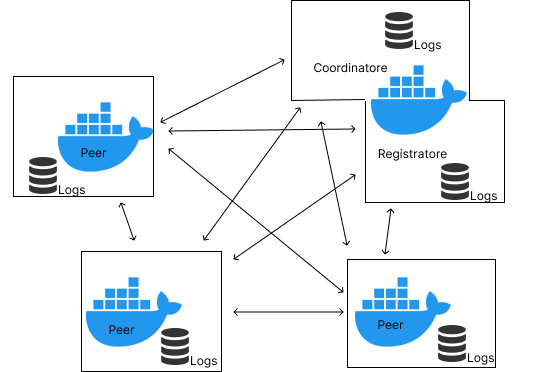
\includegraphics[width=6cm,height=6cm,keepaspectratio]{arch.png}}
\caption{Architettura dell'applicazione}
\label{fig}
\end{figure}

\section{Implementazione dei flag}

Passare dei parametri di input ad applicazioni avviate con docker-compose è stata una sfida. Ho deciso per poter passare dei flag di creare uno script bash per l'avvio dell'applicazione, che prenda i parametri di input e li salvi su un file \textit{.env}. Nel docker-compose è poi possibile specificare di prendere le variabili d'ambiente del container da questo file. Due variabili sono necessarie come input dell'applicazione, il numero di peer che parteciperanno e che dovranno essere instanziati dal docker-compose e quale algoritmo usare per l'accesso alla sezione critica. Ci sono poi due valori aggiuntivi, il flag \textit{verbose} e il flag \textit{delay}. \textit{Verbose} può essere attivato per creare dei file di log su cui i diversi componenti dell'applicazione stamperanno messaggi dettagliati riguardo la loro attività, utile per il debugging. Ho scelto di implementare questo flag tramite stampa su file invece che sul terminale per poter avere i messaggi separati in base al peer che li ha scritti, il che rende il tutto più leggibile. Ogni messaggio è accompagnato da un timestamp. L'applicazione mostra anche alcune stampe su terminale, che restano però invariate indifferente dalla modalità \textit{verbose} o meno. \textit{Delay} serve per poter specificare diverse condizioni di congestione della rete. Ci sono tre modalità possibili, si parte da una rete molto veloce fino ad arrivare a una rete abbastanza congestionata. Questo è stato implementato generando un numero random prima dell'invio di ogni messaggio tra due peer e mettendo il peer in sleep per i microsecondi specificati. I numeri random vengono specificati in tre intervalli differenti in base alla velocità che si intende simulare. Avere un sistema del genere permette anche di togliere prevedibilità alla nostra applicazione, dato che senza la generazione di numeri random esecuzioni successive con gli stessi parametri di avvio dovrebbero portare sempre allo stesso ordine di messaggi ed entrate in sezione critica, ma questo non è ciò che succede in un sistema reale. Per ottenere questo sistema non prevedibile, il generatore di numeri random viene inizializzato con il tempo corrente in nanosecondi come seme, in modo da utilizzare stream di numeri differenti ad ogni esecuzione.

\section{Testing}

Sono stati implementati tre test, uno responsabile di controllare che due processi non entrino mai in contemporanea dentro la sezione critica, uno per controllare che gli algoritmi usati garantiscano una certa fairness nel concedere l'accesso in sezione critica e uno per controllare che gli algoritmi mantengano liveness. Entrambi questi test sono scritti in go e sono basati sulla lettura e controllo automatico dei log una volta terminata un'esecuzione. I test sono eseguibili specificando se si desidera testare un gruppo con diversi peer o il caso limite di un singolo peer, specificando l'algoritmo e specificando quanto delay di rete dovrà essere presente. Anche per l'avvio dei test è stato creato uno script bash, che avvii l'applicazione, la faccia eseguire per un certo tempo, la spenga e poi vada ad eseguire i test sui file di log prodotti. Il test per controllare la mutua esclusività va a formare una lista dove ogni elemento contiene le informazioni sul peer di cui si sta parlando e i due timestamp per un'entrata in sezione critica e la rispettiva uscita. Ordinando per timestamp di entrata, si prende il primo elemento della lista e si controlla che nessuno degli elementi che lo seguono sia entrato in sezione critica in un momento precedente rispetto al suo timestamp di uscita. 
Per quanto riguarda il controllo della fairness, parte dell'assunzione che i peer richiedono l'accesso alla sezione critica ad intervalli più o meno regolari, ed essendo il ritardo di rete generato artificialmente nello stesso intervallo per ogni peer, questo significa che dovrebbe arrivare la prima richiesta da ogni peer, quando tutte sono state servite la seconda... Quindi, sapendo che le richieste arrivano in modo regolare, se verifichiamo che le entrate in sezione critica siano regolari possiamo verificare la fairness degli algoritmi. Per far questo, contiamo le entrate in sezione critica per ogni peer, e ogni volta che incrementiamo uno dei contatori controlliamo che non ci sia mai una differenza di più di due entrate tra un peer e un altro, quindi che i contatori vengano incrementati in modo simmetrico. Per quanto riguarda la liveness, il tempo più lungo per cui un algoritmo può restare bloccato senza invio di messaggi è quando un peer è in sezione critica e tutti gli altri sono in attesa di una release. Contando 10 secondi come tempo massimo passato in sezione critica e 5 secondi come tempo massimo per l'invio di un messaggio (rete molto congestionata), possiamo supporre che se tra l'ultimo messaggio ricevuto da un peer e il suo stop sono passati più di quindici secondi l'algoritmo è andato in dead-lock. Su questo è basato il test della liveness, considerando diversi tempi in base alla velocità della rete e alcuni secondi aggiuntivi come margine di errore.

\subsection*{Testing e rete congestionata}

Inizialmente ho pensato i test in modo che il test con più peer che tentano di accedere contemporaneamente alla sezione critica venisse effettuato con cinque peer, ma nel caso di rete congestionata questo ha fatto si che nel minuto di esecuzione riservato per il test le entrate in sezione critica fossero pochissime, in molti casi alcuni peer non riuscivano a entrare neanche una volta. Dato che effettuare test con tempi molto lunghi potrebbe risultare poco conveniente, ho deciso di fare il test con solo tre peer per poter avere un'esecuzione un po' più significativa.



\begin{thebibliography}{00}
\bibitem{b1} Wee k. Ng,  Chinya V. Ravischankar, "Coterie Templates: A New Quorum Construction Method", 1995
\end{thebibliography}


\end{document}
